\section{Data Link Layer}
\paragraph{Schicht 2: Sicherungsschicht}
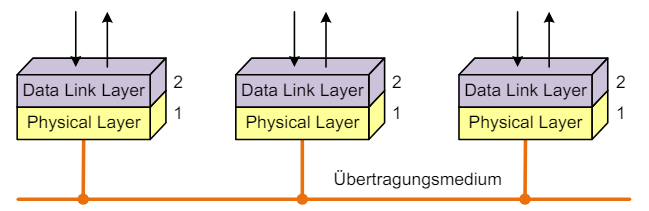
\includegraphics[width=0.5\linewidth]{images/data_link_layer.png}
\begin{definition}{Aufgaben}
    \begin{itemize}
        \item Realisieren einer zuverlässigen Verbindung zwischen Systemen
        \item Framing und Flow Control
        \item bei >2 Teilnehmern: Adressierung, Media Access, Timing
    \end{itemize}
\end{definition}

\begin{definition}{Framing (Rahmenbildung-/erkennung)}\\
    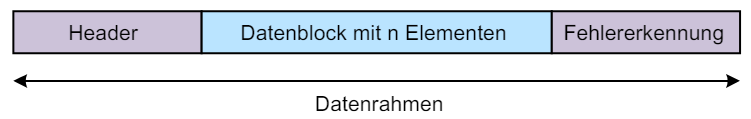
\includegraphics[width=0.6\linewidth]{images/frame_def.png}
    \begin{itemize}
        \item Senderichtung: Einpacken der zu sendenen Nutzdaten in Datenrahmen (Frames)
        \item Empfangsrichtung: Erkennung und Auspacken der Datenblöcke aus empfangenen Frames
    \end{itemize}
\end{definition}

\begin{concept}{Asynchron}\\
    Keine Daten → Nichts wird gesendet (Pause zwischen Frames)
    \begin{itemize}
        \item Zu Beginn eines Frames wird ein Start-Bit gesendet
        \item Prüfbits am Ende eines Frames!
        \item Frame-Grenze gibt auch Byte-Grenze
    \end{itemize}
    \includegraphics[width=0.7\linewidth]{images/asynchrone_übertragung_dll.png}
\end{concept}

\begin{concept}{Synchron}\\
    Frames werden ohne Unterbruch gesendet (kontinuierlicher Bitstrom auf Physical Layer)
    \begin{itemize}
        \item Stehen keine Daten an, werden Flags gesendet
    \end{itemize}
    \includegraphics[width=0.8\linewidth]{images/synchron_übertragung_dll.png}\\
    Frames werden durch ein Start-Flag und ein End-Flag begrenzt:\\
    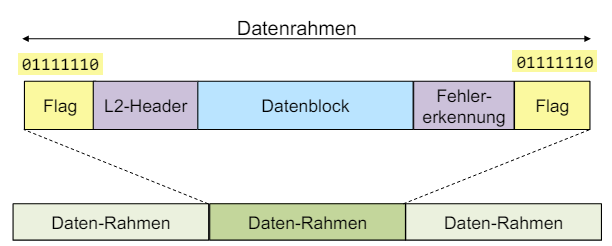
\includegraphics[width=0.6\linewidth]{images/flags_frames.png}\\
    Maskierung von Sonderzeichen (Flags) nötig!
\end{concept}

\begin{concept}{Bitstopfen}\\
    Wird verwendet um ein Bit-Muster zu garantieren.
    \begin{itemize}
        \item Sender fügt im Datenstrom nach 5 Einsen immer eine Null ein
        \item Empfänger wirft nach 5 Einsen immer ein Bit weg
        \item Somit gibt es (ausser bei Flags) die Bitfolge 01111110
    \end{itemize}
        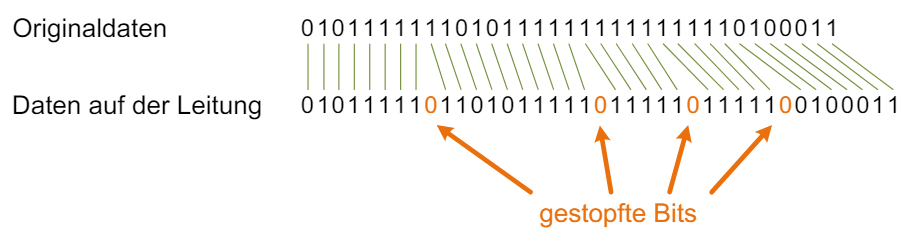
\includegraphics[width=0.7\linewidth]{images/bit_stuffing.png}
\end{concept}

\subsection{Fehlererkennung/-Korrektur}

\begin{definition}{Fehlerwahrscheinlichkeit}
    BER (Bit Error Ratio):
    \begin{itemize}
        \item Eigenschaft des Physical Layers
        \item wird als Dezimalzahl ausgedrückt: BER = 0.5 $\rightarrow$ jedes 2. Bit falsch
    \end{itemize}
    Weitere Definitionen:
    \begin{itemize}
        \item FER (Frame Error Ratio): Fehlerhaft empfangene Daten (Frames)
        \item RER (Residual Error Ratio): Unentdeckte, fehlerhaft empfangene Frames
    \end{itemize}
\end{definition}

\begin{KR}{Frame-Fehlerwahrscheinlichkeit}
    Wie gross ist die Wahrscheinlichkeit, dass ein Frame der Länge N mindestens einen Bitfehler enthält?\\
    Für BER = $p_e << 1$ gilt: $(1 - p_e)^N \approx (1 - N \cdot p_e)$ , also: 
    $$P_{Fehler, Frame} \approx N \cdot p_e (=FER)$$
\end{KR}

\begin{theorem}{Wahl der Framelänge}\\
    Die Wahl der optimalen Framegrösse ist ein Kompromiss zwischen Overhead und einer geringen Frame- und Restfehlerwahrscheinlichkeit. Sie wird von der Bitfehlerwahrscheinlichkeit, der Datenrate und Verzögerungen im System beeinflusst.
    \begin{itemize}
    \item Lange Frames:
    \begin{itemize}
        \item Höhere Nutzdatenrate (höhere Netto-Bitrate, weniger Overhead)
        \item Fehlerwahrscheinlichkeit wird grösser
        \item Datenverlust bei einem Fehler wird grösser
        \item Wahrscheinlichkeit eines unentdeckten Fehlers wird grösser
    \end{itemize}
    \item Kurze Frames: Tiefere Nutzdatenrate, Zuverlässig
    \end{itemize}
\end{theorem}



\begin{formula}{Framelänge}
    Nettobitrate = Bruttobitrate $\cdot \frac{Nutzdaten}{Nutzdaten + Header}$
\end{formula}

\begin{formula}{Datenraten}
    $$F_R = \frac{B}{8\cdot(F_L + IFG)}$$
    $F_R$ = Framerate, B = Bitrate, $F_L$ = Framelength
    $$N = F_R \cdot P \cdot 8$$
    N = Nutzbitrate, P = Payload
\end{formula}
%\textbf{Example or KR for actual exercises!!}
\begin{example}
    Gegeben: Bitrate 100 Mbit/s, Frame-Länge 1000 Byte, IFG 96 Bit, Payload 800 Byte. Berechnen Sie die Nutzdatenrate.\\
    \textbf{Lösung:}\\
    $$F_R = \frac{100 \cdot 10^6}{8 \cdot (1000 + 96)} = 1.19 \cdot 10^6 \text{ Frames/s}$$
    $$N = 1.19 \cdot 10^6 \cdot 800 \cdot 8 = 7.6 \cdot 10^9 \text{ Bit/s} = 7.6 \text{ Gbit/s}$$
\end{example}

\begin{KR}{Key Takes Fehlererkennung/Fehlerkorrektur}\\
    Zu Fehlererkennung wird den Daten Redundanz beigefügt (in Form von zusätzlich übertragener Information).
    \begin{itemize}
        \item Diese erhöht die Hamming Distanz (= Mindestanzahl unterschiedlicher Bits zwischen gültigen Codewörtern).
        \item Die betrachteten Verfahren gehören zur Familie der Block Codes.
    \end{itemize}
    Fehlerkorrektur kann rückwärtsgerichtet (Erneutes Übertragen der Daten) oder vorwärtsgerichtet (Rekonstruktion von verfälschten Bits beim Empfänger, Forward Error Correction FEC) erfolgen.
\end{KR}

\columnbreak

\subsubsection{Verfahren zur Fehlererkennung}

\begin{concept}{Fehlererkennung}\\
    Die Zuverlässigkeit der Fehlererkennung ist abhängig von der Framelänge und gewähltem Verfahren\\
    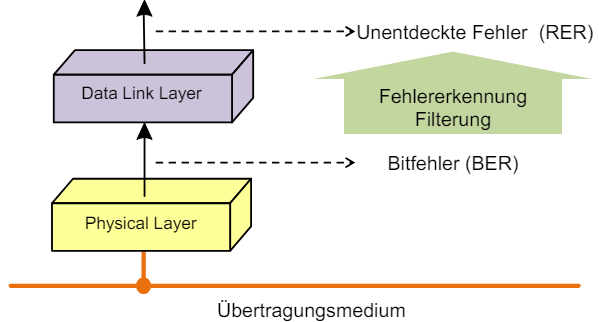
\includegraphics[width=0.5\linewidth]{images/fehlererkennung.png}\\
    Standards IEEE 802 (LAN-Standards, zb Ethernet):
    \begin{itemize}
        \item max. $5 \cdot 10^{-14}$ unentdeckte Fehler pro Frame-Byte
        \item BER $p_e \leq 10^{-8}$
        \item CRC32 für Ethernet, mit Generatorpolynom
    \end{itemize}
\end{concept}



\begin{concept}{Hammingdistanz als Mass für Fehlerdetektion}\\
    Codes mit Hamming-Distanz $\leqq$ 2 erlauben die Erkennung von Ein- oder Mehr-Bitfehlern \\
        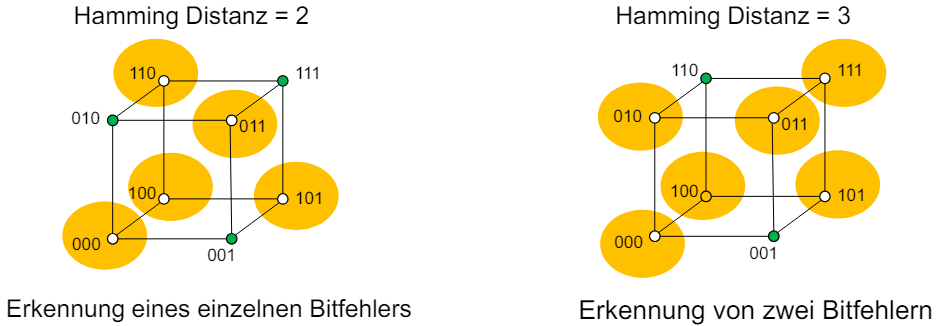
\includegraphics[width=0.8\linewidth]{images/hamming_distanz.png}\\
    Generelle Regel für Hamming-Distanz h: erlaubt Erkennung von (h-1) Fehlern 
    $$e = h - 1$$
\end{concept}

\begin{concept}{Fehlererkennung mit einfacher Parity}\\
    Ein (1) Prüfbit sichert ein Datenwort (typisch 1 Byte, auch 7 oder 9 Bits werden verwendet)\\
        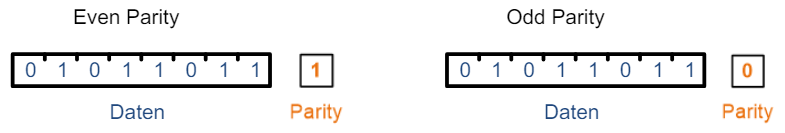
\includegraphics[width=0.8\linewidth]{images/einfache_parity.png}
\begin{itemize}
    \item Even Parity: Anzahl 1er inkl. Parity-Bit ist gerade
    \item Odd Parity: Anzahl 1-Bit inklusive Parity-Bit ist ungerade
\end{itemize}
Even und Odd Parity sind gleichwertig
\end{concept}

\begin{concept}{Längs- und Quer-Parity}\\
        \includegraphics[width=0.6\linewidth]{images/längs-quer-parity.png}\\
    Wie viele Fehler können korrigiert/erkannt werden?
    \begin{itemize}
        \item Korrigieren: 1 Bit-Fehler
        \item Erkennen: mind. 3 Bit-Fehler
    \end{itemize}
\end{concept}



\subsubsection{Zugriffsmechanismen (Media Access)}

\paragraph{Gesteuerter Medium Zugriff}

\begin{definition}{Master-Slave Verfahren}\\
    Verwenden mehrere Systeme das gleiche physikalische Medium, so muss der Zugriff auf das Medium koordiniert werden\\
        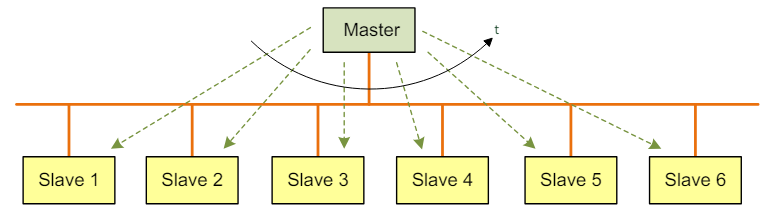
\includegraphics[width=0.75\linewidth]{images/master-slave.png}
    \begin{itemize}
        \item Vorteil: Keine Konflikte, Master koordiniert Zugriff
        \item Nachteil: Ausfall des Masters (Single Point of Failure)
    \end{itemize}
\end{definition}

\begin{definition}{Token Verfahren}\\
    Die Sendeberechtigung wird in einer festgelegten Reihenfolge weitergereicht: Knoten senden nur, wenn sie ein Token halten\\
        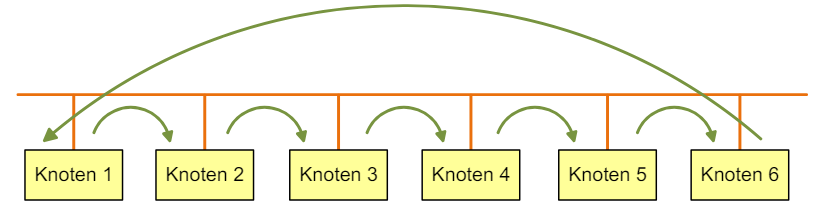
\includegraphics[width=0.75\linewidth]{images/token-verfahren.png}
    \begin{itemize}
        \item Vorteil:  Deterministisch (man weiss, wann man dran kommt)
        \item Nachteil: Aufwändig (Startup, Token Verlust, etc.)
    \end{itemize}
\end{definition}

\begin{concept}{Kombi Master-Slave und Token}\\
    Variante: Anstelle eines Tokens wird ein Frame geschickt
    \begin{itemize}
        \item Knoten fügen ihre Daten an den vorbestimmten Positionen ein (Interbus, Ethercat) oder hängen die Daten hinten am Frame an (PROFINET Dynamic Frame Packing)
        \item Typische Anwendung in einer Master/Slave-Konfiguration
    \end{itemize}
        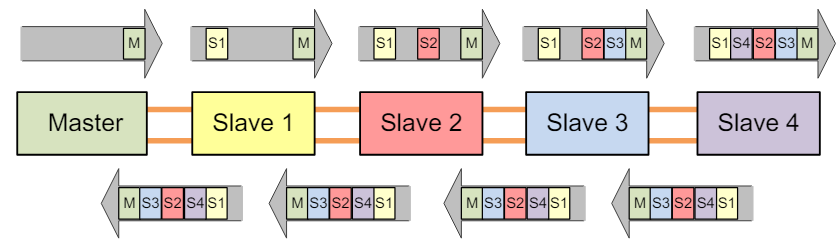
\includegraphics[width=0.75\linewidth]{images/combo_master_slave_token.png}
\end{concept}

\begin{definition}{Zeitsteuerung}\\
    Zeitgesteuerter Zugriff (Netzbetrieb analog Taktfahrplan im Bahnnetz)
    \begin{itemize}
        \item Vorteil: Optimierung möglich (nach Auslastung, Durchsatz, «Reisezeit» etc.)
        \item Nachteile:
        \begin{itemize}
            \item Planung und genaue Zeit in allen Knotepunkten erforderlich
            \item Konflikte mit unplanbarem Verkehr (SBB Cargo)
        \end{itemize}
        \item Anwendungen: PROFINET IRT, Time Sensitive Networks
    \end{itemize}
\end{definition}

\paragraph{Random Medium Zugriff}

\begin{definition}{Carrier Sense Multiple Access}
    Vorteil: Alle Stationen sind gleichberechtigt (kein Master) und haben jederzeit Zugriff auf das Übertragungsmedium
    \begin{itemize}
        \item Vor dem Senden wird das geteilte Übertragungsmedium abgehört, ob es frei ist (Carrier Sense), sonst wird bis zu einer Pause gewartet.
    \end{itemize}
        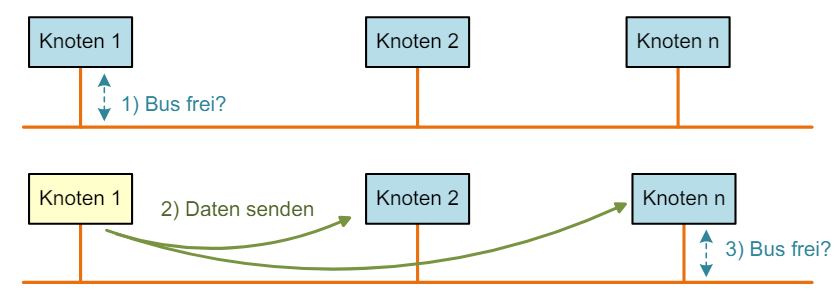
\includegraphics[width=0.75\linewidth]{images/random_access_thingy.png}\\
    Frage: Was geschieht, wenn 2 Knoten gleichzeitig warten und zum Schluss kommen, dass sie senden können?
\end{definition}

\begin{concept}{Kollisionsbehandlung}\\
    Für die Kollisionsbehandlung gibt es verschiedene Möglichkeiten:
    \begin{itemize}
        \item CSMA/CD (Collision Detection): Abbrechen und später nochmals Versuchen
        \begin{itemize}
            \item Originalmechanismus im Ethernet, heute praktisch nicht mehr verwendet
        \end{itemize}
        \item CSMA/CR (Collision Resolution): Hardware-unterstütze Arbitrierung
        \begin{itemize}
            \item Arbitierung kann passiv sein (wie unten) oder aktiv (via Busmaster)
            \item Anwendung: CAN-Bus
        \end{itemize}
    \end{itemize}
        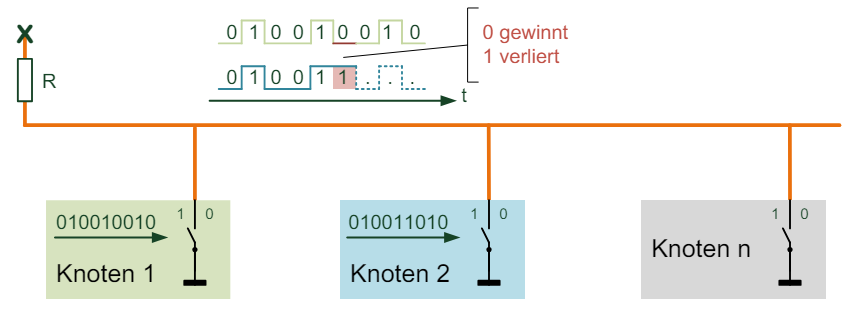
\includegraphics[width=0.75\linewidth]{images/kollisionsbehandlung.png}
\end{concept}

\begin{KR}{Key Takes Zugriffsmechanismen und Flow Control}
\begin{itemize}
    \item Bei mehr als 2 Kommunikationsteilnehmern (Shared Medium) benötigt es auf dem Data Link ein Verfahren zur Adressierung und zur Steuerung der Sendeberechtigung (Medium Access).
    \begin{itemize}
        \item Master/Slave, Token-, Zeitgesteuert, oder mit Kolissionserkennung und –auflösung.
    \end{itemize}
    \item Flusskontrolle wird im Zusammenhang mit Ende-zu-Ende Flusskontrolle Schicht 4 behandelt, ist aber auch Aufgabe von Schicht 2 (falls implementiert).
\end{itemize}
\end{KR}

\subsection{Flow Control}

\begin{definition}{Explizite Start-Stop Signalisierung}
    \begin{itemize}
        \item Flow Control erlaubt einem Empfänger den Sender temporär zu stoppen
        \item Die Stop-/ Start-Meldungen können über Leitungen oder Meldungen im Datenrückkanal erfolgen (siehe Praktikum 2).
        \item Anwendungen:
        \begin{itemize}
            \item Empfänger mit langsamer Verarbeitung
            \item .. und mit zu wenig Memory um den ganzen Verkehr zu speichern
            \item Verstopfungen im Netzwerk (Überlastsituationen)
        \end{itemize}
    \end{itemize}
        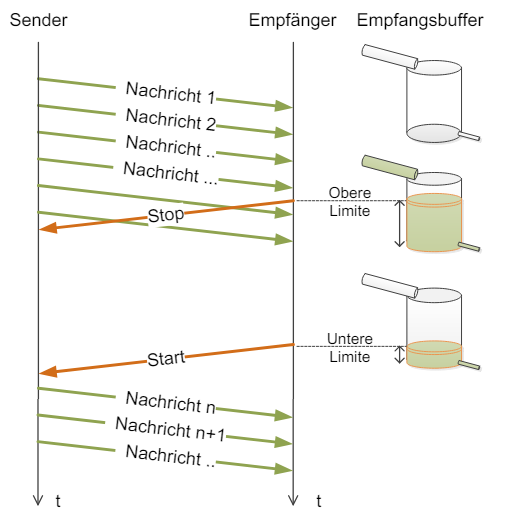
\includegraphics[width=0.5\linewidth]{images/flow_control1.png}
\end{definition}

\begin{definition}{Implizit mit Stop and Wait Protokoll}\\
    Flow Control ist quasi «gratis», wenn ein Stop-and-Wait-Protokoll für die Backward Error Correction verwendet wird:
    \begin{itemize}
        \item Sender wartet auf Quittung
        \item Empfänger verzögert seine Quittierung und stoppt damit die Übertragung
    \end{itemize}
        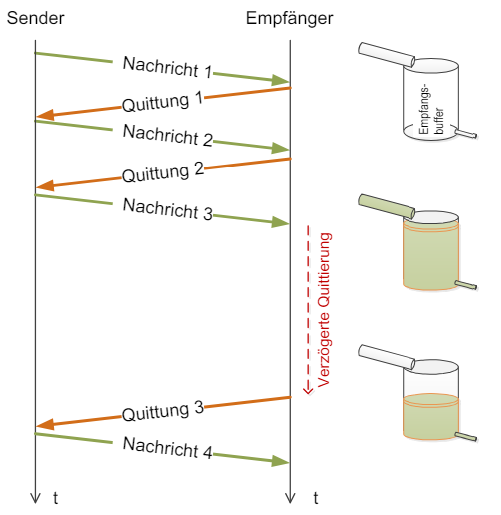
\includegraphics[width=0.5\linewidth]{images/flow_control2.png}
\end{definition}

